\chapter{Resultados e Discussões}	

A caracterização do arcabouço estrutural utilizando métodos sismológicos possui problemas de unicidade de solução, como outros métodos geofísicos.  Essa falta de informação direta do objeto em estudo proporciona uma gama de soluções. Porém há inúmeros meios de se contornar tal situação. A modelagem mostra se a técnica tem resolução para seu objetivo.

Para delimitar as principais feições utilizou-se de modelos simples, como visto na Figura \ref{modelagem}-a, apenas com camadas planas, com esses modelos pode-se mostrar que as estimativas da espessura crustal e são consistentes com os dados observados. Na modelagem utilizou-se os programas "\textit{icmod}", "\textit{icmod}", "\textit{vplot[s]}", "\textit{respknt}",  e "\textit{pwaveqn}", disponibilizados por \cite{Ammon_waterlevel_1997}.

\begin{figure}[!ht]
\centering
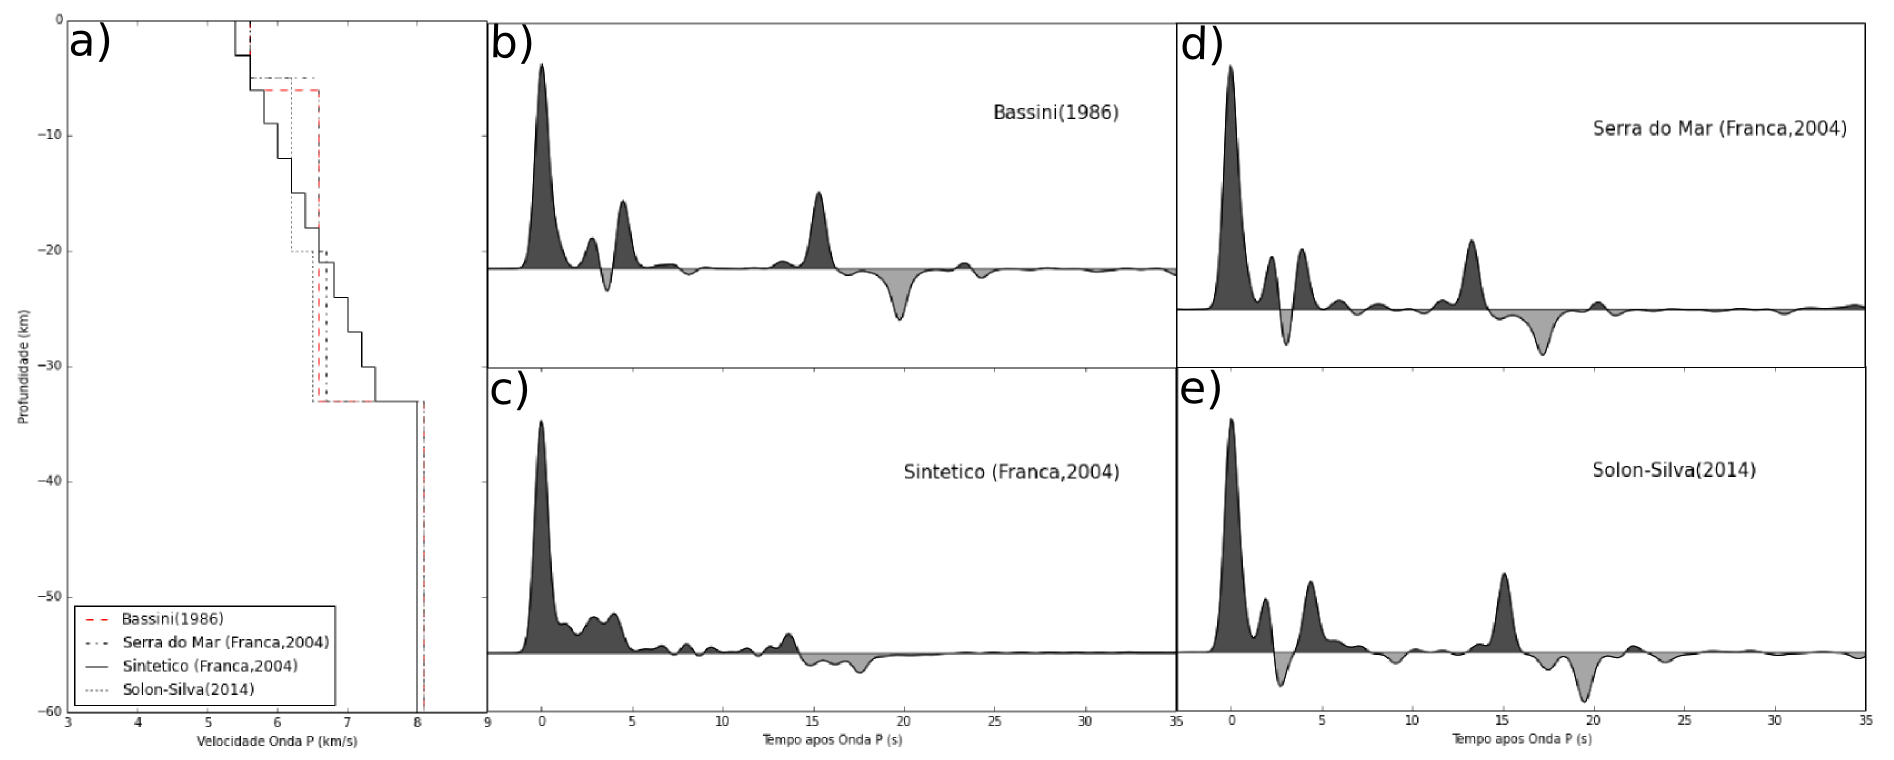
\includegraphics[scale=0.4]{modelagem_RF.png}
\caption{}
\label{modelagem}
\end{figure}


A Figura \ref{RF_perfil_NW} mostra uma seção de Funções do Receptor obtidas de vários eventos oriundos das região Noroeste. Estes sinais estão normalizados pela amplitude do primeiro pico. O primeiro pick é a chegada da onda P direta, já o segundos, por volta de 5 segundos, e a onda P convertida em onda S na discontinuidade de Moho.

\begin{figure}[!ht]
\centering
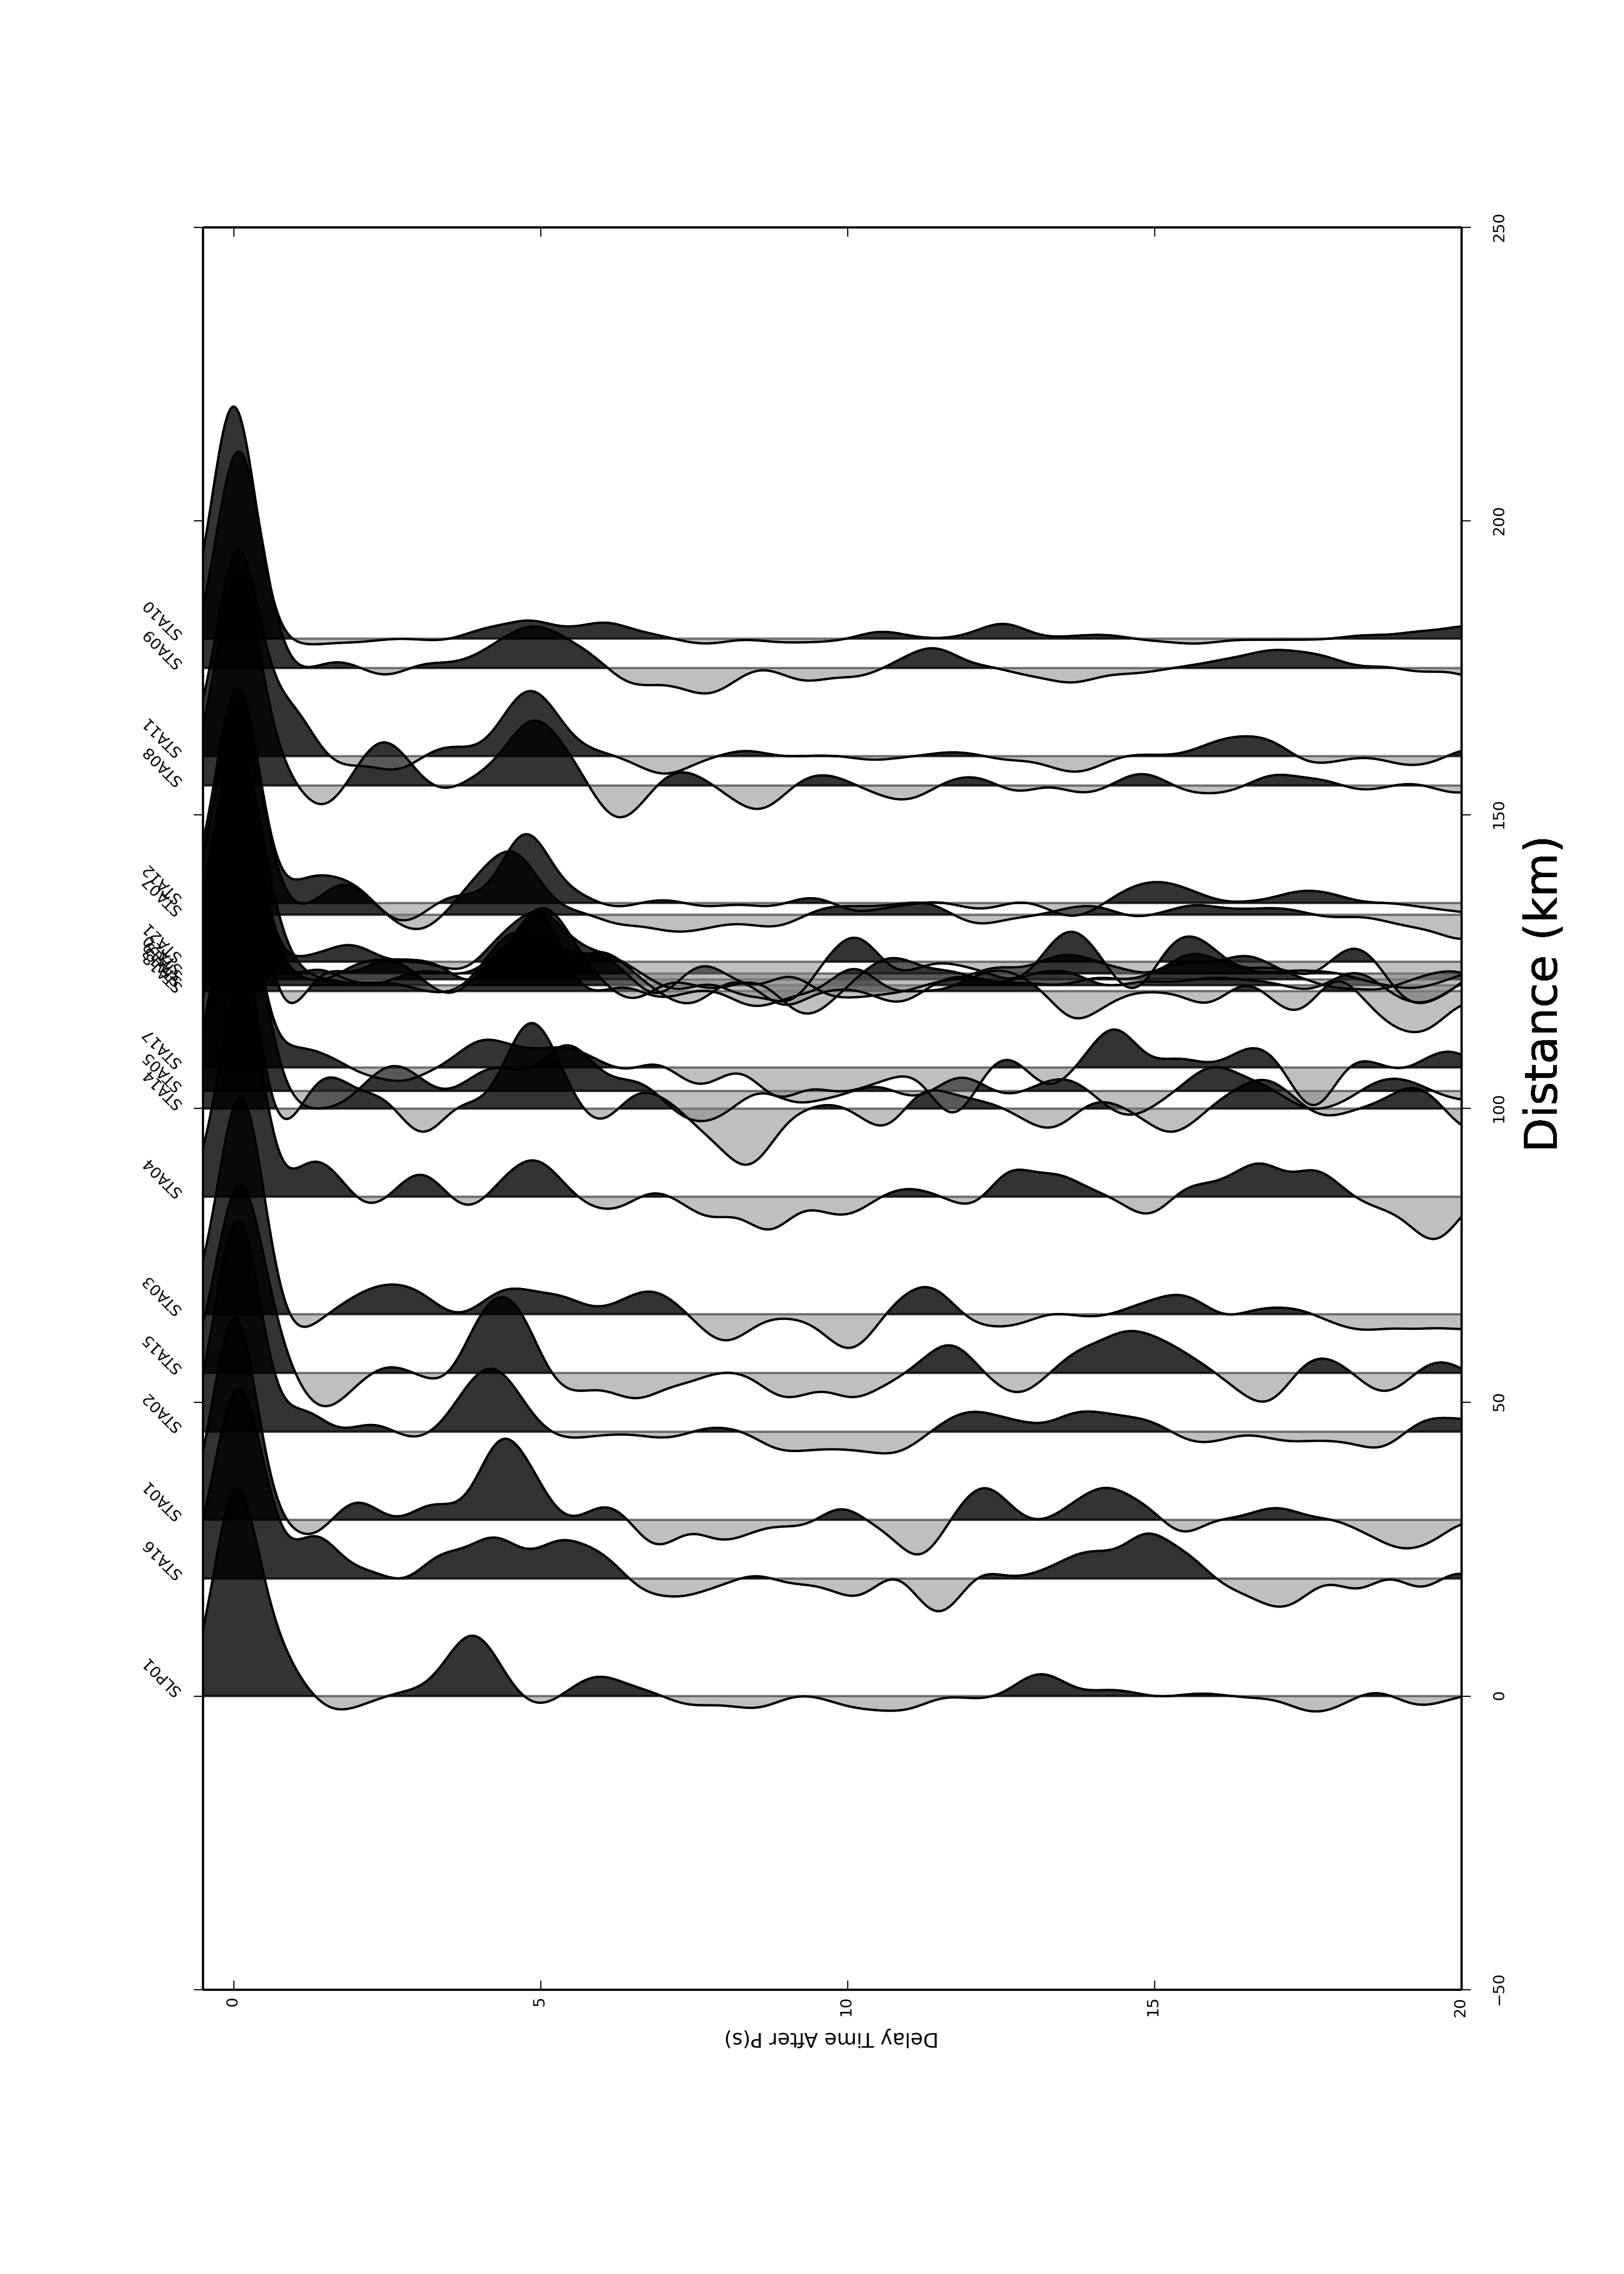
\includegraphics[scale=0.15]{Perfil_RF_NWLS.png}
\caption{}
\label{RF_perfil_NW}
\end{figure}


As multiplas $PpPs$ e $PpSs+PsPs$ tem uma amplitude menor que a onda P convertida em S($Ps$). Nota-se na Figura \ref{RF_perfil_NW} que a discontinuidade de Moho estimada é maior no interior do continente do que na região costeira, corroborando com os dados de \cite{Assumpcao_America_2013}, \citep{Assumpcao_Brazil_2013} e \cite{van_der_meijde_gravity_2013} . Identfica-se sinais precursores a Moho, por volta de 2 a 4 segundos, que variam ao longo do perfil. Estes sinais podem ser relacionados com uma interface com um alto contraste de propriedade fisica. O pulso negativo antes de 5 segundos indica, segundo as modelagens propostas na Figura \ref{modelagem}, uma camada com baixa velocidade.





The uncertainties of data are linked to the quality and the quantity of the Receiver Functions. The estimated values of the Moho depth for each station were linearly interpolated to generate a regional map, shown in Figure. In order to improve the interpolation, we added data from \citep{assumpcao_crustal_2013}. In Figure \ref{figura7}, we can see the Moho thinning in direction to the east.

The Figure \ref{figura5} shows a section of Receiver Functions obtained from several events and normalized by the amplitude of the first peak. The first peak is the direct P-wave arrival, the second highest, around 5 seconds, is the P wave converted to S wave in the Moho discontinuity. 





The uncertainty, shown in Table \ref{tabela} are linked to quality and quantity of the Receiver Functions. A important phase is the selection of the best Receiver Functions, because the data quality is preponderant over the quantity. The uncertainty associated a each one of obtained parameters by the method Hk and estimated generally by "bootstrap" method, developed for  \citep{efron_statistical_1991}. From the original set of Receiver Functions the program generates subsets containing traces randomly selected. These method is repeated for each subsets, resulting in a parameter set H and $v_{p}/v_{s}$ .Mean and standard deviation from the values provide us a mean value and an estimate of the uncertainty associated to determination. There is no rule for determining the number subsets that must be generated, the crucial is search a value that makes the estimative stabilize,  including uncertainties. In general we use a value between 100 and 200 subsets depending on the amount de traces available during the “bootstrap”.

The calculated values of the Moho depth for each station were linearly interpolated to generate a regional map, shown in the Figure \ref{figura7}. To improve the interpolation, we added data from \citep{assumpcao_crustal_2013}. In the Figure \ref{figura7} we can see the Moho thinning in direction to east, reinforcing the proximity with the oceanic crust.

